\documentclass[10pt]{article}
\usepackage{graphicx,amsmath,amssymb,bm}
\usepackage{amsfonts}

\begin{document}

\section*{Master thesis project for H\aa kon Vik\o r Treider: Multiscale physics}

The aim of a program on multiscale physics is to develop a first
principle approach to systems of relevance for a variety of fields,
from materials science to nano-technology and biological systems and
even atomic nuclei and stars.  Common to all these systems is that
they entail a truly multiscale physics program that involves a proper
understanding of the links between the various scales, starting from
quantum-mechanical first principle studies of atoms, molecules and
eventually other spatially confined systems to Density functional
theories and finally microscopically derived potentials to be used in
molecular dynamics calculations.

The computations required for accurate modeling and simulation of large-scale
systems with atomistic resolution involve a hierarchy of levels of theory: quantum
mechanics (QM) to determine the electronic states; force fields to average the
electronics states and to obtain atom based forces (FF), molecular dynamics (MD)
based on such an FF; mesoscale or coarse grain descriptions that average or
homogenize atomic motions; and finally continuum level descriptions.
By basing computations on first principles QM it is possible to overcome the
lack of experimental data to carry out accurate predictions with atomistic resolu-
tion, which would otherwise be impossible. Furthermore, QM provides the funda-
mental information required to describe quantum effects, electronically excited
states, as well as reaction paths and barrier heights involved in chemical reactions
processes. However, the practical scale for accurate QM today is <1,000 atoms per
molecule or periodic cell (a length scale of a few nanometers) whereas the length
scale for modeling supramolecular systems in biology may be in the tens of nano-
meters, while elucidating the interfacial effects between grains in composite materials
may require hundreds of nanometers, and modeling turbulent fluid flows or shock-
induced instabilities in multilayered materials may require micrometers. Thus,
simulations of engineered materials and systems may require millions to billions
of atoms, rendering QM methods impractical.
Nonetheless, QM methods are essential for accurately describing atomic-level
composition, structure and energy states of materials, considering the influence of
electronic degrees of freedom. By incorporating time-dependent information, the
dynamics of a system under varying conditions may be explored from QM-derived
forces, albeit within a limited timescale (<1 ps). The prominent challenge for theory
and computation involves efficiently bridging, from QM first-principles, into larger
length scales with predominantly heterogeneous spatial and density distributions,
and longer timescales of simulation – enough to connect into engineering-level
design variables – while retaining the appropriate accuracy and certainty. Equally
challenging remains the inverse top-down engineering design problem, by which
macroscopic material/process properties would be tunable from optimizing its
atomic-level composition and structure. The aim of this large project is to 
to develop breakthrough methods to staple and extend hierarchically over existing
to develop the necessary tools to enable continuous lateral (multi-paradigm) 
and hierarchical (multiscale) couplings, between the different theories
and models as a function of their length- and timescale range – a strategy often referred to
as First-Principles-Based Multiscale-Multiparadigm Simulation.
The enclosed figure here displays some of these ideas.
\begin{figure}[thbp]
  \begin{center}
    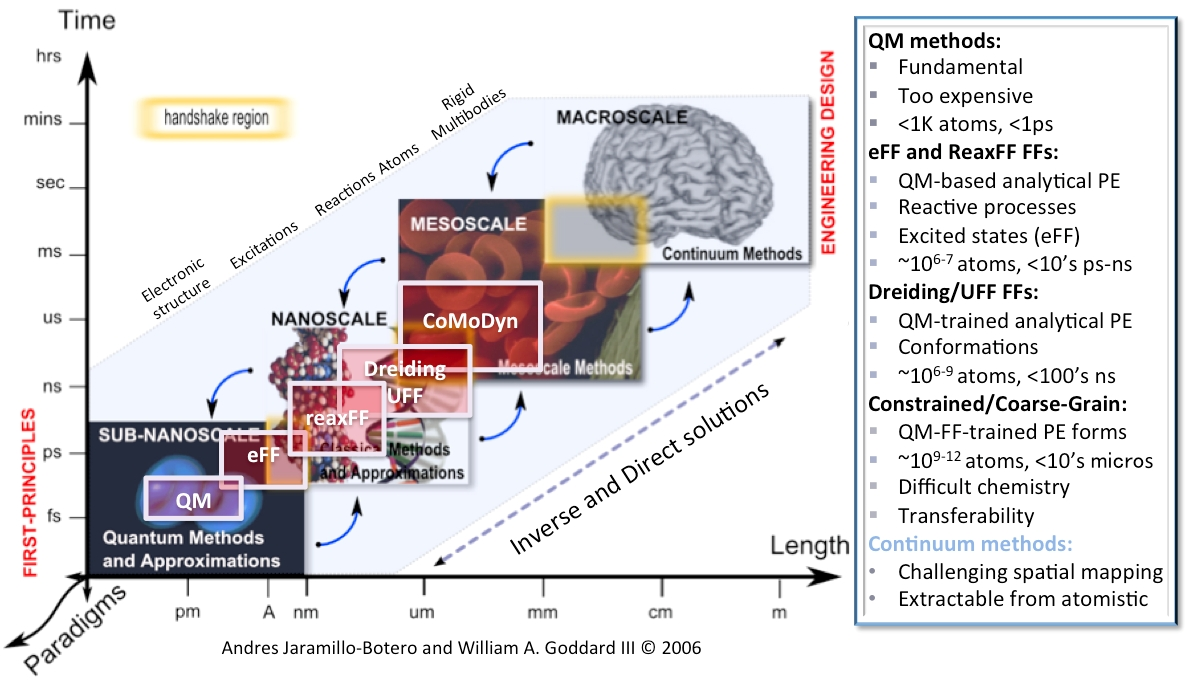
\includegraphics[width=0.75\textwidth,clip=]{multiscale.jpg}
  \end{center}
  \caption{Example of multiscale hierarchy.}
  \label{fig1}
\end{figure}
The ultimate goal is a reversible bottom-up, top-down approach, based on first
principles QM, to characterize properties of materials and processes at a hierarchy
of length and timescales. This will improve our ability to design, analyze, and
interpret experimental results, perform model-based prediction of phenomena, and
to control precisely the multi-scale nature of material systems for multiple applications. 

To achieve these goals, several theses projects are shortly defined below. These projects open also up for
several fruitful collaborations between the involved MSc students. The group in Computational Physics has long-standing
experience in defining projects where several students may find a common a ground, either from a formalism point of view or (and possibly and as well) phenomenological point of view.

The systems we have in mind are mainly molecules like SiO$_2$, H$_2$O,
CaCO$_3$ and other more complicated molecules. To model the
interaction between such molecules and eventually derive microscopic
interactions can be done via several MSc projects. 
The aim of this thesis is to perform quantum-mechanical first principle calculations of selected molecules 
compounds and compare these results with parametrized potential model like the
so-called ReaxFF potential. 

\section*{Progress plan and milestones}
The aims and progress plan of this thesis are as follows
\begin{itemize}
\item Spring 2016 and partly fall 2016:  The first step is to set up a Hartree-Fock program for the H$_2$ molecule and parametrize an effective potential for molecular dynamics calculations. These results will be compared to exisiting potential models.
\item Fall 2016:  The next step is to include a proper treatment of quantum mechanical effects by performing Coupled-cluster theory  theory calculations to determine better correlations.
\item Spring 2017: The final step is to obtained parametrized potentials for more complex molecules and use these
in molecular dynamics calculations.
\end{itemize}
 
The thesis is expected to be handed in May/June 2017.





\end{document}






\documentclass[10pt]{article}
\usepackage{graphicx,amsmath,amssymb,bm}
\usepackage{amsfonts}

\begin{document}

\section*{Multiscale physics, from quantum mechanical simulations of atoms and molecules to molecular dynamics}

What is presented here is a large project which involves several Master theses  projects. 
The various projects are listed below, opening up for several possibilities.

The aim of a program on multiscale physics is to develop a 
first principle approach to systems of relevance for a variety of fields, from materials science to nano-technology and biological systems and even
atomic nuclei  and stars. 
Common to all these systems is that they entail a truly multiscale physics program that involves a proper understanding of the links
between the various scales, starting 
from quantum-mechanical first principle studies of atoms, molecules and eventually other spatially confined 
systems to Density functional theories and finally microscopically derived potentials to be used in molecular dynamics calculations. 

The computations required for accurate modeling and simulation of large-scale
systems with atomistic resolution involve a hierarchy of levels of theory: quantum
mechanics (QM) to determine the electronic states; force fields to average the
electronics states and to obtain atom based forces (FF), molecular dynamics (MD)
based on such an FF; mesoscale or coarse grain descriptions that average or
homogenize atomic motions; and finally continuum level descriptions.
By basing computations on first principles QM it is possible to overcome the
lack of experimental data to carry out accurate predictions with atomistic resolu-
tion, which would otherwise be impossible. Furthermore, QM provides the funda-
mental information required to describe quantum effects, electronically excited
states, as well as reaction paths and barrier heights involved in chemical reactions
processes. However, the practical scale for accurate QM today is <1,000 atoms per
molecule or periodic cell (a length scale of a few nanometers) whereas the length
scale for modeling supramolecular systems in biology may be in the tens of nano-
meters, while elucidating the interfacial effects between grains in composite materials
may require hundreds of nanometers, and modeling turbulent fluid flows or shock-
induced instabilities in multilayered materials may require micrometers. Thus,
simulations of engineered materials and systems may require millions to billions
of atoms, rendering QM methods impractical.
Nonetheless, QM methods are essential for accurately describing atomic-level
composition, structure and energy states of materials, considering the influence of
electronic degrees of freedom. By incorporating time-dependent information, the
dynamics of a system under varying conditions may be explored from QM-derived
forces, albeit within a limited timescale (<1 ps). The prominent challenge for theory
and computation involves efficiently bridging, from QM first-principles, into larger
length scales with predominantly heterogeneous spatial and density distributions,
and longer timescales of simulation – enough to connect into engineering-level
design variables – while retaining the appropriate accuracy and certainty. Equally
challenging remains the inverse top-down engineering design problem, by which
macroscopic material/process properties would be tunable from optimizing its
atomic-level composition and structure. The aim of this large project is to 
to develop breakthrough methods to staple and extend hierarchically over existing
to develop the necessary tools to enable continuous lateral (multi-paradigm) 
and hierarchical (multiscale) couplings, between the different theories
and models as a function of their length- and timescale range – a strategy often referred to
as First-Principles-Based Multiscale-Multiparadigm Simulation.
The enclosed figure here displays some of these ideas.
\begin{figure}[thbp]
  \begin{center}
    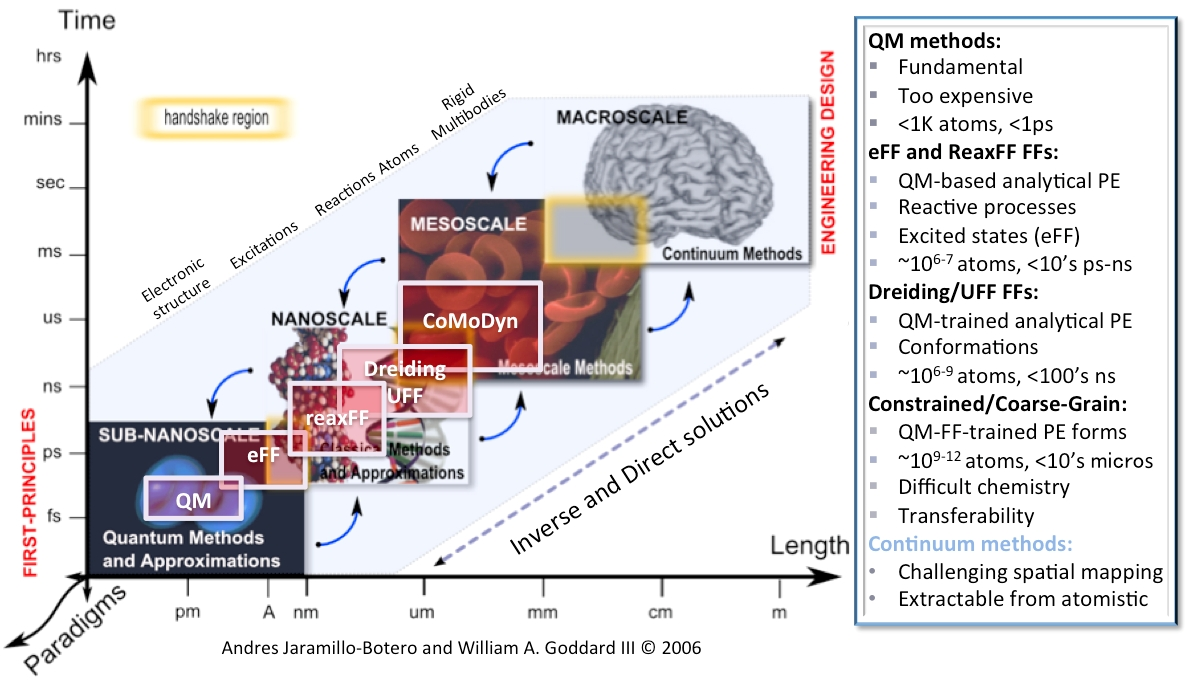
\includegraphics[width=0.75\textwidth,clip=]{multiscale.jpg}
  \end{center}
  \caption{Example of multiscale hierarchy.}
  \label{fig1}
\end{figure}
The ultimate goal is a reversible bottom-up, top-down approach, based on first
principles QM, to characterize properties of materials and processes at a hierarchy
of length and timescales. This will improve our ability to design, analyze, and
interpret experimental results, perform model-based prediction of phenomena, and
to control precisely the multi-scale nature of material systems for multiple applications. 

To achieve these goals, several theses projects are shortly defined below. These projects open also up for
several fruitful collaborations between the involved MSc students. The group in Computational Physics has long-standing
experience in defining projects where several students may find a common a ground, either from a formalism point of view or (and possibly and as well) phenomenological point of view.

There are several possible projects. The systems we have in mind are mainly molecules 
\begin{itemize}
\item Start with exisiting codes and thesis work by previous Master of Science students at the 
computational physics group. Here we think in particular of using existing Hartree-Fock codes for atoms and molecules and use these to develop potential surfaces and thereby extract parametrized potentils for molecular dynamics calculations. One possible path is to start with a gas of hydrogen and compare the parametrized potentials from Hartree-Fock theory with exisiting models, as done in the thesis of Svenn-Arne Dragly \url{https://www.duo.uio.no/handle/10852/41843}. 
\item Quantum mechanical correlations are however treated only approximatively in Hartree-Fock theory. Monte Carlo methods offer a path to cpmpute exactly ground state properties of correlated quantum mechanical systems. Here one can use existing (developed at the Computational Physics group) or develop a variational and diffusion Monte Carlo code that computes properties such as binding energies, root mean square radii, charge
distributions and local potentials.  This topic can easily form the basis for one or two  MSc thesis projects. These first principle approaches can be used to develop potential surfaces, which in turn 
can be used to parametrize potentials for molecular dynamics studies.
\item If more complex atoms and molecules are involved, one may consider freezing the inner degrees of freedom using for example
many-body perturbation theory to derive an effective interaction for electrons outside a chosen core. Alternatively one can use existing coupled cluster codes (also part of the computational quantum mechanics codes developed at the computational physics group) to derive potential surfaces and thereby parametrize potentials to use in molecular dynamics calculations.
\item The quantum mechanical  calculations can in turn be used to define better density functionals for the above atoms. Density functional theory can in turn
be used to study for example lattices of atoms and molecules with say periodic boundary conditions.
\item 
These effective potentials
can in turn be compared with existing models such as the so-called  ReaxFF potential. The implementation and studies of this potential for 
studies of say  SiO$_2$ compounds
could form the basis  for one or two  MSc thesis projects. 
\end{itemize}



\end{document}















